\documentclass[11pt]{article}

% ============================================================================
%  Kasami permutation criterion -- the REFACTORED library
%  A paper-to-Lean map organised by mathematical role, with the module DAG
%  and the Dobbertin(1999) <-> library correspondence.
% ============================================================================

\usepackage[a4paper,margin=2.3cm]{geometry}
\usepackage{amsmath,amssymb,amsthm}
\usepackage{xcolor}
\usepackage{framed}
\usepackage{listings}
\usepackage{tikz}
\usetikzlibrary{arrows.meta,positioning,shapes.geometric,fit,backgrounds,calc,shapes.multipart}
\usepackage{tikz-cd}
\usepackage{enumitem}
\usepackage[hidelinks]{hyperref}
\usepackage{caption}
\usepackage{longtable}
\usepackage{fontspec}
\setmonofont{DejaVu Sans Mono}

% ---------------------------------------------------------------------------
%  Colours
% ---------------------------------------------------------------------------
\definecolor{leanbg}{RGB}{245,247,250}
\definecolor{leanframe}{RGB}{200,210,222}
\definecolor{leankw}{RGB}{150,20,120}
\definecolor{leancmt}{RGB}{90,120,90}
\definecolor{leanstr}{RGB}{160,80,20}
\definecolor{quotebar}{RGB}{40,90,160}
\definecolor{mathlibcol}{RGB}{215,232,255}
\definecolor{fieldcol}{RGB}{222,245,222}
\definecolor{numcol}{RGB}{224,240,255}
\definecolor{mapcol}{RGB}{255,244,214}
\definecolor{critcol}{RGB}{235,225,255}
\definecolor{headcol}{RGB}{255,224,224}

% ---------------------------------------------------------------------------
%  Lean listing style
% ---------------------------------------------------------------------------
\lstdefinelanguage{lean4}{
  morekeywords={theorem,lemma,def,noncomputable,variable,namespace,end,open,
    import,scoped,in,by,fun,if,then,else,do,with,match,let,have,show,from,
    calc,intro,intros,exact,apply,rw,rwa,simp,simp_all,ring,ring_nf,omega,
    omit,convert,using,refine,obtain,rcases,rintro,constructor,funext,
    set,unfold,cases,induction,at,Prop,Type,Function,structure,instance,
    grind,decide,linarith,nlinarith,linear_combination,field_simp,aesop,
    tauto,by_contra,exfalso,contrapose,use},
  sensitive=true,
  morecomment=[l]{--},
  morecomment=[s]{/-}{-/},
  morestring=[b]",
}
\lstset{
  language=lean4,
  basicstyle=\ttfamily\footnotesize,
  keywordstyle=\color{leankw}\bfseries,
  commentstyle=\color{leancmt}\itshape,
  stringstyle=\color{leanstr},
  backgroundcolor=\color{leanbg},
  frame=single,
  rulecolor=\color{leanframe},
  framesep=5pt,
  xleftmargin=6pt,
  xrightmargin=2pt,
  breaklines=true,
  breakatwhitespace=false,
  columns=fullflexible,
  keepspaces=true,
  showstringspaces=false,
}
\protected\def\lc#1{\texttt{\detokenize{#1}}}

% ---------------------------------------------------------------------------
%  Paper-quote environment
% ---------------------------------------------------------------------------
\newenvironment{paperquote}[1]
 {\par\smallskip\noindent
  \def\FrameCommand{\color{quotebar}\vrule width 3pt\hspace{8pt}}%
  \MakeFramed{\advance\hsize-\width \FrameRestore}%
  \small\itshape
  \noindent\normalfont\footnotesize\textbf{\textsf{Dobbertin (1999) --- #1}}\par\nobreak\smallskip\itshape}
 {\endMakeFramed\par\smallskip}

\theoremstyle{definition}
\newtheorem{correction}{Correction}
\newtheorem*{remark}{Remark}

\title{\textbf{The Kasami Permutation Criterion --- a refactored Lean\,4 library}\\[4pt]
\large Module map, dependency DAG, and Dobbertin\,(1999) correspondence,\\[2pt]
\normalsize organised by mathematical role rather than by paper numbering}
\author{Formalisation library \texttt{KasamiPermutations.*}}
\date{}

\begin{document}
\maketitle

\begin{abstract}
\noindent
This document describes the \emph{refactored} Lean\,4 library
\texttt{KasamiPermutations.*}, which formalises --- from the \texttt{Mathlib}
foundations, end to end and \texttt{sorry}-free --- the opening of
H.~Dobbertin's \emph{Theorem~1} (\emph{Kasami Power Functions, Permutation
Polynomials and Cyclic Difference Sets}, 1999, pp.~133--138): equation~(1), the
permutation criterion for the generalized Kasami map $q_\alpha$, and the first
substantive step $(1)\Rightarrow(2)$.  The refactoring reorganises the modules
\emph{by mathematical role} (a Frobenius theory, a trace theory, a Mersenne
number-theory fact, the Kasami-map definitions, and two permutation criteria)
rather than by their numbering in the paper, following the ``small, coherent,
reusable module'' principle.  We give the module dependency DAG, the
old\,$\to$\,new rename map, and a declaration-level Dobbertin\,$\leftrightarrow$\,Lean
correspondence, and we record the simplifications made.  Every headline result
rests only on the standard axioms \lc{propext}, \lc{Classical.choice},
\lc{Quot.sound}.
\end{abstract}

\tableofcontents
\bigskip

% ===========================================================================
\section{The refactoring at a glance}
% ===========================================================================

The library proves, for $L=\mathbb F_{2^n}$ with $\gcd(k,n)=1$, $k<n$ and
$k\,k'\equiv 1\pmod n$, that the generalized Kasami map
\[
   q_\alpha(z)=\Bigl(\textstyle\sum_{i=1}^{k'} z^{2^{ik}}+\alpha\,\mathrm{Tr}(z)\Bigr)
   \cdot z^{(2^n-1)-(2^k+1)}
   \qquad(\alpha\in\{0,1\})
\]
is a permutation of $L$ \emph{iff} $k'+\alpha n\equiv 1\pmod 2$, and that
equation~(1),
\[
   c\,x^{2^k+1} \;=\; \sum_{i=1}^{k'} x^{2^{ik}} \;+\; \alpha\,\mathrm{Tr}(x),
   \tag{1}
\]
implies the linearized equation~(2)
$\;\ell(x)=c^{2^k}x^{2^{2k}}+x^{2^k}+cx+1=0$.

\paragraph{Organizing principle.}
The previous layout named files and namespaces after the paper's numbering
(\texttt{Theorem5}, \texttt{Theorem8Trace}, \texttt{Theorem8C1},
\texttt{Q1General}, \texttt{Equation1}, \texttt{Defs}, \texttt{Setup},
\texttt{FiniteFieldPrereqs}).  The refactored layout instead groups declarations
by \emph{what they are about}, so that each module is a small, self-describing,
independently reusable theory:

\begin{itemize}[leftmargin=1.4em,itemsep=2pt]
\item a \textbf{Frobenius} theory and a \textbf{trace} theory of a finite
      field of characteristic $2$ (upstreamable, Kasami-agnostic);
\item a \textbf{Mersenne number-theory} fact (upstreamable, field-agnostic);
\item the \textbf{Kasami-map definitions} and their \textbf{special values};
\item the two \textbf{permutation criteria} --- one for the constant-bit map
      $q^{(\varepsilon)}$, one for the trace map $g=q_1$ --- and the
      \textbf{headline} assembly with the $(1)\Rightarrow(2)$ step.
\end{itemize}

% ===========================================================================
\section{Old\,$\to$\,new rename map}
% ===========================================================================

\renewcommand{\arraystretch}{1.25}
\begin{longtable}{@{}p{0.30\linewidth}p{0.32\linewidth}p{0.30\linewidth}@{}}
\hline
\textbf{Old file / namespace} & \textbf{New file / namespace} & \textbf{Mathematical role}\\
\hline
\endhead
\lc{Defs.lean}\newline\lc{Dobbertin1999.Paper} &
\lc{KasamiMap.lean}\newline\lc{Kasami} &
definitions of $\mathrm{Tr}$, $q_\alpha$, eqn~(1), $\ell$, $Q$\\
\lc{Setup.lean} (values) &
\lc{SpecialValues.lean}\newline\lc{Kasami} &
$q_\alpha(0)$, $q_\alpha(1)$; the ``only if'' direction\\
\lc{Setup.lean} (arithmetic) &
\lc{NumberTheory/MersenneNumbers.lean}\newline\lc{Kasami.NumberTheory} &
$\gcd(2^k{-}1,2^n{-}1)$ and modular inverse\\
\lc{FiniteFieldPrereqs.lean} (Frobenius) &
\lc{FiniteField/Frobenius.lean}\newline\lc{Kasami.FiniteField} &
Frobenius $x\mapsto x^{p^r}$ facts\\
\lc{FiniteFieldPrereqs.lean} (trace) \newline $+$ \lc{Theorem8Trace.lean} \newline $+$ \lc{Theorem8C1.lean} (trace) &
\lc{FiniteField/Trace.lean}\newline\lc{Kasami.FiniteField} &
additive/absolute trace and its identities\\
\lc{Theorem5.lean}\newline\lc{Dobbertin.Thm5} &
\lc{TraceFreeCriterion.lean}\newline\lc{Kasami.TraceFreeCriterion} &
criterion for the constant-bit map $q^{(\varepsilon)}$\\
\lc{Q1General.lean}\newline\lc{Dobbertin.Thm8C1Gen} \newline $+$ \lc{Theorem8C1.lean} (\lc{gmap}) &
\lc{TraceVersionCriterion.lean}\newline\lc{Kasami.TraceVersionCriterion} &
criterion for the trace map $g=q_1$\\
\lc{Equation1/Equation1.lean}\newline\lc{Dobbertin1999.Paper} &
\lc{PermutationCriterion.lean}\newline\lc{Kasami} &
headline criterion for $q_\alpha$; $(1)\Rightarrow(2)$\\
\hline
\end{longtable}

\noindent The headline declarations were also renamed to describe the pattern
they prove:

\renewcommand{\arraystretch}{1.2}
\begin{center}
\begin{tabular}{@{}lll@{}}
\hline
\textbf{Old name} & \textbf{New name} & \textbf{Statement}\\
\hline
\lc{theorem_5} & \lc{qeps_bijective_iff} & $q^{(\varepsilon)}$ bijective $\iff \varepsilon\equiv k'{+}1$\\
\lc{theorem_1} & \lc{qKasami_bijective_iff} & $q_\alpha$ bijective $\iff k'{+}\alpha n$ odd\\
\lc{theorem_1_case1} & \lc{linearized_root_unique} & $\ell(x)=0$ has a unique root (case 1)\\
\lc{theorem_1_case2} & \lc{eqn1_nonzero_root_unique} & eqn~(1) has a unique nonzero root (case 2)\\
\lc{gmap_bijective_iff} & \lc{gmap_bijective_iff} & $g=q_1$ bijective $\iff k'{+}n$ odd\\
\lc{eqn2_of_eqn1} & \lc{eqn2_of_eqn1} & $(1)\Rightarrow(2)$\\
\hline
\end{tabular}
\end{center}

% ===========================================================================
\section{Module dependency DAG}
% ===========================================================================

Every import points ``upward'' in the DAG below; reading the modules in
topological order is the same as reading the mathematics from the foundations
up.  The number-theory fact and the special values form the small
``opening/only-if'' branch that is independent of the main root-count argument.

\begin{center}
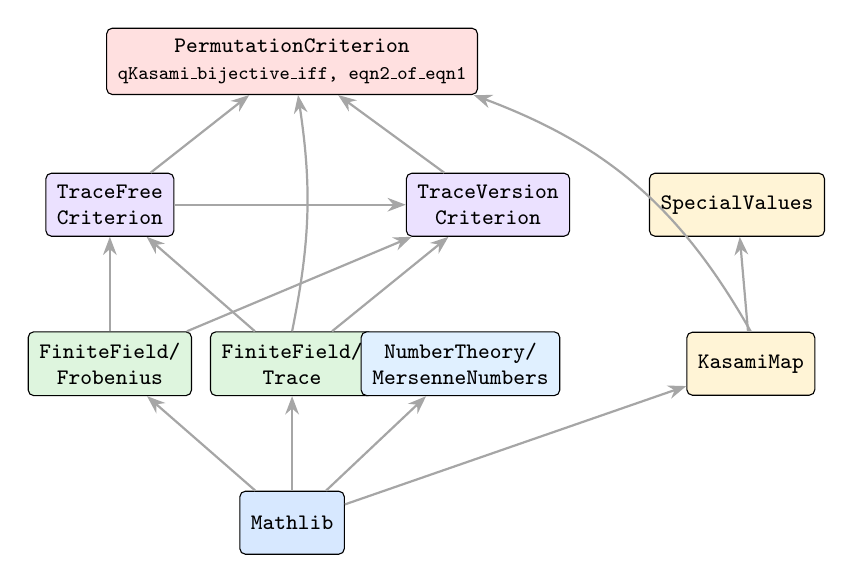
\begin{tikzpicture}[
  >=Stealth, node distance=7mm,
  box/.style={draw, rounded corners=2pt, align=center, font=\footnotesize\ttfamily,
              inner sep=4pt, minimum height=8mm},
  ml/.style={box, fill=mathlibcol},
  ff/.style={box, fill=fieldcol},
  nt/.style={box, fill=numcol},
  mp/.style={box, fill=mapcol},
  cr/.style={box, fill=critcol},
  hd/.style={box, fill=headcol},
  dep/.style={->, thick, gray!70}
]
\node[ml] (ml) {Mathlib};

\node[ff, above left=12mm and 6mm of ml] (frob) {FiniteField/\\Frobenius};
\node[ff, above=12mm of ml] (trace) {FiniteField/\\Trace};
\node[nt, above right=12mm and 2mm of ml] (mers) {NumberTheory/\\MersenneNumbers};
\node[mp, right=16mm of mers] (kmap) {KasamiMap};

\node[cr, above=12mm of frob] (tfc) {TraceFree\\Criterion};
\node[cr, above right=12mm and 4mm of trace] (tvc) {TraceVersion\\Criterion};
\node[mp, right=10mm of tvc] (sv) {SpecialValues};

\node[hd, above=30mm of trace] (perm) {PermutationCriterion\\ \scriptsize qKasami\_bijective\_iff, eqn2\_of\_eqn1};

\draw[dep] (ml) -- (frob);
\draw[dep] (ml) -- (trace);
\draw[dep] (ml) -- (mers);
\draw[dep] (ml) -- (kmap);
\draw[dep] (frob) -- (tfc);
\draw[dep] (trace) -- (tfc);
\draw[dep] (frob) -- (tvc);
\draw[dep] (trace) -- (tvc);
\draw[dep] (tfc) -- (tvc);
\draw[dep] (kmap) -- (sv);
\draw[dep] (tfc) -- (perm);
\draw[dep] (tvc) -- (perm);
\draw[dep] (trace.north) to[bend right=10] (perm);
\draw[dep] (kmap.north) to[bend right=20] (perm);
\end{tikzpicture}
\end{center}

\noindent
\textbf{Colour key:}\quad
\colorbox{mathlibcol}{\scriptsize Mathlib}\quad
\colorbox{fieldcol}{\scriptsize finite-field theory}\quad
\colorbox{numcol}{\scriptsize number theory}\quad
\colorbox{mapcol}{\scriptsize Kasami definitions}\quad
\colorbox{critcol}{\scriptsize criteria}\quad
\colorbox{headcol}{\scriptsize headline}.

% ===========================================================================
\section{The foundation layer: finite-field and number theory}
% ===========================================================================

\subsection{\texttt{FiniteField/Frobenius} --- the Frobenius endomorphism}

A Kasami-agnostic theory of the map $x\mapsto x^{p^r}$ on a finite field.

\begin{lstlisting}
namespace Kasami.FiniteField
lemma frob_cycle (x : F) : x ^ Fintype.card F = x
lemma frob_mod (hn : Fintype.card F = p ^ n) (x : F) (r : ℕ) :
    x ^ (p ^ r) = x ^ (p ^ (r % n))
lemma frob_bijective (r : ℕ) : Function.Bijective (fun x : F => x ^ (p ^ r))
lemma pow_field_bijective (ha : Nat.Coprime (Fintype.card F - 1) a) (ha_pos : 0 < a) :
    Function.Bijective (fun x : F => x ^ a)
\end{lstlisting}

These package Fermat's little theorem (\lc{FiniteField.pow_card}), Frobenius
injectivity (\lc{iterateFrobenius_inj}) and the pigeonhole ``injective
$\Rightarrow$ surjective'' device (\lc{Finite.injective_iff_surjective}).

\subsection{\texttt{FiniteField/Trace} --- the additive (absolute) trace}

\begin{paperquote}{p.~135, trace properties}
$\mathrm{Tr}(x)=\mathrm{Tr}(x^2)$ and $\mathrm{Tr}(x)\in\{0,1\}$; the absolute
trace is $\mathbb F_2$-linear.
\end{paperquote}

\begin{lstlisting}
namespace Kasami.FiniteField
def truncTrace (m : ℕ) (x : F) : F := ∑ i ∈ Finset.range m, x ^ (2 ^ i)
lemma truncTrace_add : truncTrace m (x + y) = truncTrace m x + truncTrace m y
lemma truncTrace_sq_add_self : truncTrace m x ^ 2 + truncTrace m x = x ^ (2 ^ m) + x
theorem trace_frob_shift (hn) (k) (x) : truncTrace n (x ^ (2 ^ k)) = truncTrace n x
theorem trace_artin_schreier_zero (hn) (k) (t) : truncTrace n (t ^ (2 ^ k) + t) = 0
theorem trace_sq  (hn) (x) : (truncTrace n x) ^ 2 = truncTrace n x
theorem trace_bit (hn) (x) : truncTrace n x = 0 ∨ truncTrace n x = 1
\end{lstlisting}

\begin{remark}
This single module now collects trace facts that were previously scattered
across three files (\lc{FiniteFieldPrereqs}, \lc{Theorem8Trace},
\lc{Theorem8C1}).  \lc{truncTrace_add} is the ``freshman's dream''
(\lc{add_pow_char_pow}); \lc{truncTrace_sq_add_self} is the telescoping identity;
\lc{trace_frob_shift}/\lc{trace_artin_schreier_zero} are the paper's Frobenius
invariance and Artin--Schreier vanishing; and \lc{trace_sq}/\lc{trace_bit}
express $\mathrm{Tr}(x)\in\{0,1\}$.
\end{remark}

\subsection{\texttt{NumberTheory/MersenneNumbers}}

\begin{paperquote}{p.~135, opening of the proof}
First note that $(2^k-1)^{-1}\pmod{2^n-1}$ exists, since $\gcd(k,n)=1$.
\end{paperquote}

\begin{lstlisting}
namespace Kasami.NumberTheory
theorem mersenne_coprime (h : Nat.Coprime k n) :
    Nat.Coprime (2 ^ k - 1) (2 ^ n - 1)
theorem inv_mod_exists (h : Nat.Coprime k n) (hn : 1 < 2 ^ n - 1) :
    ∃ b, (2 ^ k - 1) * b % (2 ^ n - 1) = 1
\end{lstlisting}

The key Mathlib input is $\gcd(2^k-1,2^n-1)=2^{\gcd(k,n)}-1$
(\lc{Nat.pow_sub_one_gcd_pow_sub_one}).

% ===========================================================================
\section{The Kasami map and its special values}
% ===========================================================================

\subsection{\texttt{KasamiMap} --- the definitions}

\begin{lstlisting}
namespace Kasami
def Tr (n : ℕ) (x : L) : L := ∑ i ∈ Finset.range n, x ^ (2 ^ i)
def qKasami (n k k' α : ℕ) (z : L) : L :=
  ((∑ i ∈ Finset.Icc 1 k', z ^ (2 ^ (i * k))) + (α : L) * Tr n z)
    * z ^ (2 ^ n - 1 - (2 ^ k + 1))
def eqn1 (n k k' α : ℕ) (c x : L) : Prop :=
  c * x ^ (2 ^ k + 1) = (∑ i ∈ Finset.Icc 1 k', x ^ (2 ^ (i * k))) + (α : L) * Tr n x
def ell  (k : ℕ) (c x : L) : L := c ^ (2 ^ k) * x ^ (2 ^ (2 * k)) + x ^ (2 ^ k) + c * x + 1
def Qmap (k : ℕ) (c γ x : L) : L := c * x ^ (2 ^ k) + γ ^ 2 * x + γ
\end{lstlisting}

\subsection{\texttt{SpecialValues} --- the ``only if'' direction}

\begin{paperquote}{p.~135}
We have $q_\alpha(0)=0$; and $k'+\alpha n\equiv 0\pmod 2$ is equivalent to
$q_\alpha(1)=k'\cdot 1+\alpha\,\mathrm{Tr}(1)=0$.
\end{paperquote}

\begin{lstlisting}
namespace Kasami
theorem qKasami_zero (α) : qKasami n k k' α 0 = 0
theorem qKasami_one  (α) : qKasami n k k' α 1 = ((k' + α * n : ℕ) : L)
theorem qKasami_one_eq_zero_iff (α) :
    qKasami n k k' α 1 = 0 ↔ (k' + α * n) % 2 = 0
\end{lstlisting}

% ===========================================================================
\section{The two permutation criteria}
% ===========================================================================

\subsection{\texttt{TraceFreeCriterion} (paper: Theorem 5)}

\begin{paperquote}{Theorem 5, p.~137}
$q^{(\varepsilon)}$ is a permutation polynomial on $L$ if and only if
$\varepsilon\equiv k'+1\pmod 2$.
\end{paperquote}

\begin{lstlisting}
namespace Kasami.TraceFreeCriterion
def qeps (n k k' : ℕ) (ε x : F) : F := (sTrace k k' x + ε) * x ^ (2 ^ n - 1 - (2 ^ k + 1))
theorem qeps_bijective_iff (hn) (hk0) (hkn) (hcop) (hkk') (hexp) (hε : ε = 0 ∨ ε = 1) :
    Function.Bijective (qeps n k k' ε) ↔ (ε = 1 ↔ Even k')
\end{lstlisting}

The proof reduces $q^{(\varepsilon)}(x)=c$ (for a fixed value $c$) to the
linearized equation $\ell(x)=0$ by adding to it its $2^k$-th power
(\lc{ell_of_eq}), and then counts roots via a case split
(\lc{root_count}, \lc{Q_factor}, \lc{ell0_root_imp_image}).

\subsection{\texttt{TraceVersionCriterion} (paper: Theorem 8)}

Here the constant bit $\varepsilon$ is replaced by the actual trace $\mathrm{Tr}(x)$,
giving the map $g(x)=q^{(\mathrm{Tr}\,x)}(x)$, i.e.\ the $\alpha=1$ object $q_1$.

\begin{lstlisting}
namespace Kasami.TraceVersionCriterion
noncomputable def gmap (n k kk : ℕ) (x : F) : F := qeps n k kk (truncTrace n x) x
theorem gmap_bijective_iff (hn) (hk0) (hkn) (hcop) (hkk') (hexp) :
    Function.Bijective (gmap n k kk) ↔ Odd (kk + n)
\end{lstlisting}

The three admissible parities of $(k',n)$ (they are never both even, since
$\gcd(k',n)=1$) are handled uniformly through the single criterion
$\mathrm{Odd}(k'+n)$; the proof mirrors the trace-free root count with the trace
now carried along by \lc{trace_artin_schreier_zero} and \lc{trace_bit}.

% ===========================================================================
\section{The headline: \texttt{PermutationCriterion}}
% ===========================================================================

\subsection{The permutation criterion for $q_\alpha$}

\begin{paperquote}{Theorem 1 (first part), p.~135}
$q_\alpha$ is a permutation of $L=\mathbb F_{2^n}$ if and only if
$k'+\alpha n\equiv 1\pmod 2$.
\end{paperquote}

\begin{lstlisting}
namespace Kasami
theorem qKasami_bijective_iff (hn) (hk) (hcop) (hk') (hk0) (hexp)
    (α) (hα : α = 0 ∨ α = 1) :
    Function.Bijective (qKasami n k k' α) ↔ (k' + α * n) % 2 = 1
\end{lstlisting}

The two bridge lemmas \lc{qKasami_zero_eq_qeps} and \lc{qKasami_one_eq_gmap}
identify the paper's $q_\alpha$ with the library objects \lc{qeps} (for
$\alpha=0$) and \lc{gmap} (for $\alpha=1$), so that
\lc{qKasami_bijective_iff} is assembled directly from \lc{qeps_bijective_iff}
and \lc{gmap_bijective_iff}:

\begin{center}
\begin{tikzcd}[column sep=huge,row sep=small]
q^{(\varepsilon)}\ \text{criterion} \arrow[r,"\ \alpha=0\ "] & q_\alpha\ \text{criterion} & g=q_1\ \text{criterion} \arrow[l,"\ \alpha=1\ "']
\end{tikzcd}
\end{center}

\noindent(In Lean: \lc{qeps_bijective_iff} and \lc{gmap_bijective_iff}
assemble \lc{qKasami_bijective_iff}.)

\subsection{The step $(1)\Rightarrow(2)$}

\begin{paperquote}{p.~135--136}
Adding to (1) its $2^k$-th power yields
$\ell(x)=c^{2^k}x^{2^{2k}}+x^{2^k}+cx+1=0.$ \hfill (2)
\end{paperquote}

\begin{lstlisting}
namespace Kasami
theorem eqn2_of_eqn1 (hn) (hkk1 : k * k' % n = 1) (α) (c x : L)
    (hx : x ≠ 0) (h : eqn1 n k k' α c x) : ell k c x = 0
\end{lstlisting}

\begin{correction}
The naive statement is \emph{false} at $x=0$: there the cleared equation~(1)
holds vacuously ($0=0$) while $\ell(0)=1\neq 0$.  The faithful statement adds the
hypothesis $x\neq 0$ (and the field hypotheses used by the Artin--Schreier
telescoping).  Likewise \lc{eqn1_nonzero_root_unique} counts the \emph{nonzero}
solutions of eqn~(1), because $x=0$ always solves the cleared equation; this
requires $c\neq 0$.  Both corrections are documented in the sources.
\end{correction}

\subsection{The root count (two cases)}

\begin{center}
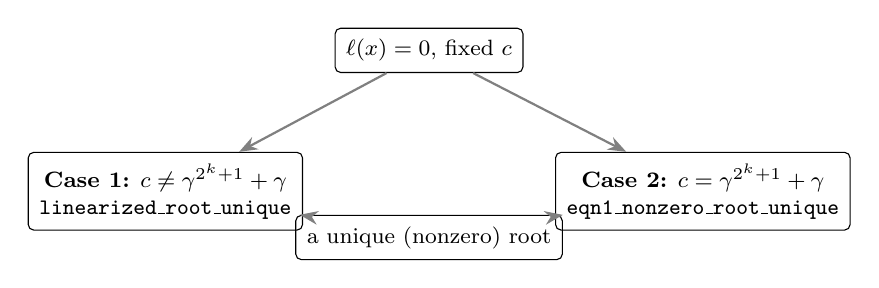
\begin{tikzpicture}[>=Stealth,node distance=5mm,
  n/.style={draw,rounded corners=2pt,align=center,font=\footnotesize,inner sep=4pt}]
\node[n] (root) {$\ell(x)=0$, fixed $c$};
\node[n, below left=10mm and 4mm of root] (c1) {\textbf{Case 1:} $c\neq\gamma^{2^k+1}+\gamma$\\ \ttfamily linearized\_root\_unique};
\node[n, below right=10mm and 4mm of root] (c2) {\textbf{Case 2:} $c=\gamma^{2^k+1}+\gamma$\\ \ttfamily eqn1\_nonzero\_root\_unique};
\node[n, below=18mm of root] (uniq) {a unique (nonzero) root};
\draw[->,thick,gray] (root) -- (c1);
\draw[->,thick,gray] (root) -- (c2);
\draw[->,thick,gray] (c1) -- (uniq);
\draw[->,thick,gray] (c2) -- (uniq);
\end{tikzpicture}
\end{center}

% ===========================================================================
\section{What the whole development reduces to}
% ===========================================================================

Stripped to the non-trivial mathematical inputs, the entire library bottoms out
on a small number of Mathlib results:
\begin{itemize}[leftmargin=1.4em,itemsep=1pt]
\item \lc{FiniteField.pow_card} (Fermat) and \lc{iterateFrobenius_inj} --- the
      Frobenius engine;
\item \lc{add_pow_char_pow} (freshman's dream) --- all char-2 telescoping;
\item \lc{Nat.pow_sub_one_gcd_pow_sub_one} --- the Mersenne-gcd fact;
\item \lc{Finite.injective_iff_surjective} --- pigeonhole ``injective
      $\Rightarrow$ permutation'';
\item \lc{Set.ncard_eq_one} --- ``exactly one solution''.
\end{itemize}
The routine char-2 algebra on top of these is discharged by the general tactics
(\lc{ring}, \lc{simp}, \lc{grind}, \lc{decide}, \lc{omega}).

% ===========================================================================
\section{Simplifications made in the refactoring}
% ===========================================================================

\begin{itemize}[leftmargin=1.4em,itemsep=2pt]
\item \textbf{Merged the trace theory.}  The scattered trace lemmas
      (freshman's dream, telescoping, Frobenius invariance, Artin--Schreier
      vanishing, idempotence/bit) now live in one \lc{FiniteField/Trace} module,
      under one namespace, so a consumer imports a single coherent theory.
\item \textbf{Split the prerequisites by concept.}  Frobenius facts and trace
      facts, previously in one \lc{FiniteFieldPrereqs} file, are now separate,
      independently reusable modules.
\item \textbf{Isolated the number theory.}  \lc{mersenne_coprime}/%
      \lc{inv_mod_exists} are field-agnostic and now sit in their own
      \lc{NumberTheory} module, ready to upstream.
\item \textbf{Named declarations after their content.}  Paper-numbered names
      (\lc{theorem_5}, \lc{theorem_1}, \dots) became statement-describing names
      (\lc{qeps_bijective_iff}, \lc{qKasami_bijective_iff}, \dots); the
      \lc{gmap} definition now lives with the criterion that uses it.
\item \textbf{Tidied proofs.}  Removed a leftover \lc{exact?}, dropped unused
      section variables and simp arguments.  No proof was weakened and the
      axiom footprint is unchanged.
\end{itemize}

\end{document}
